\documentclass[a4paper,11pt]{article}
\usepackage[a4paper, left=1.7cm, right=1.7cm, top=2cm, bottom=2cm]{geometry}
\usepackage{graphicx}

\title{Interim Report C Project Group 64}
\author{Ng Shi Hao, Rayan Abdallah, Ryan Wong, Rahul Babu}
\date{5 June 2026}

\begin{document}

\maketitle

\section{Division of Labour for Emulator}
\subsection{Ng Shi Hao}
Wrote the Makefile, binary loading, instruction fetching, and Branch-instruction module. Implemented the main fetch-decode-execute loop by tying rest of codebase together. Took responsibility for majority of codebase debugging to bring preliminary codebase onto fully passing the test suite. Conducted majority of code-refactoring, by splitting up large, dirty functions into smaller helper functions, and DRY for header problems. 
\subsection{Rayan Abdallah}
Wrote the Single Data Transfer instructions and the helper functions such as bitmasks in a pair-programming effort with Ryan. Looked through each others' PRs and tidied the codebase. 
\subsection{Ryan Wong}
Wrote the Data Processing Immediate, Data Processing Register and Bitwise Shifts instructions in a pair-programming effort with Rayan. 
\subsection{Rahul Babu}
Contributed to the logic for Branch Instructions, programming with Shi Hao.
\section{Assessment of Current Teamwork}
The team has collaborated effectively through pair-programming and regular code review. We used GitLab branches for separate tasks and feature implementation; and avoided committing directly to \texttt{master}, instead we merge completed, polished features through merge-requests. This helped us catch bugs early and made it easier to review each, separate  modules in a compartmentalized manner. \\ \\
An area for improvement is coordination around shared helper functions. Throughout the week, different members implemented similar utilities independently, leading to duplicate code. We resolved these through comprehensive discussions during group meetings and code-refactoring. Hence, for the assembler (Part II), we plan to conform towards shared interfaces early-on. 

\section{Emulator Structure}
\begin{figure}
    \centering
    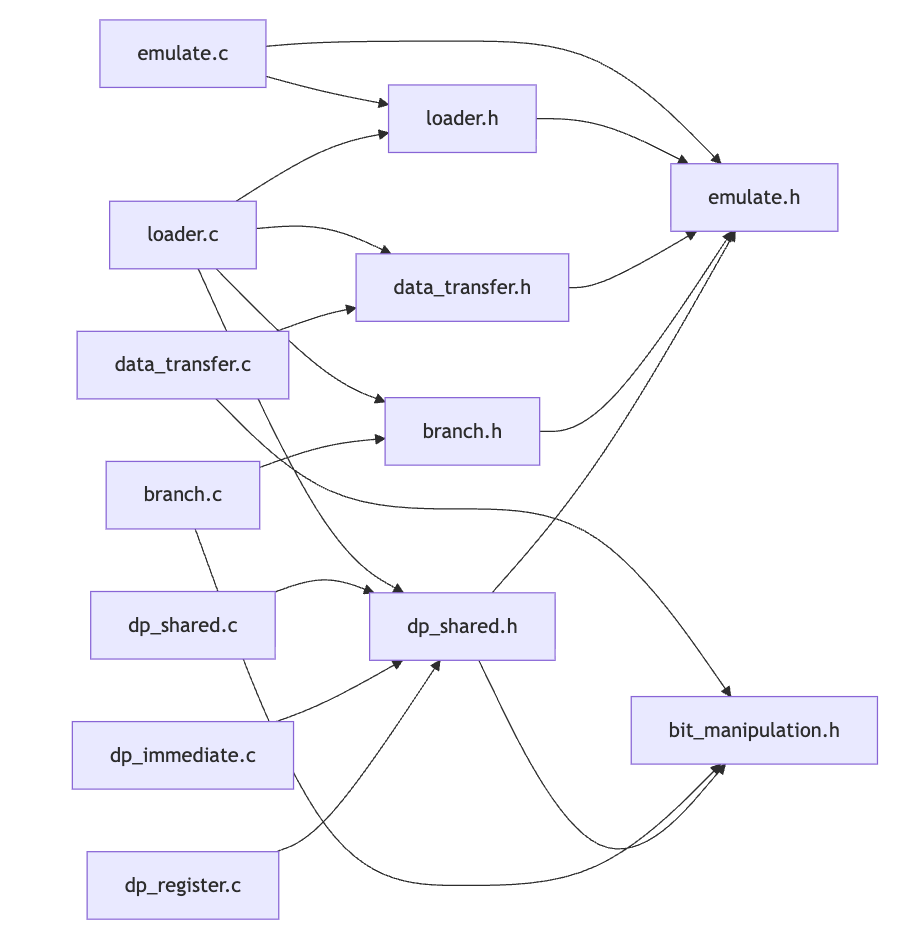
\includegraphics[width=0.6\linewidth]{Emulator-Dependencies.png}
    \caption{Dependency Graph of Emulator}
    \label{fig:placeholder}
\end{figure}
The main function for the emulator is written in \texttt{emulate.c}, which parses the input arguments, initializes emulator machine-state, loads input binary, and runs the fetch-decode-execute-loop before writing the final state. The fetch-decode-execute loop is written inside \texttt{loader.c}, which fetches instructions from memory, decodes the top-level instruction type. Then, using a switch table, the instructions are sorted by instruction type and delegated to functions in the \texttt{data\_transfer}, \texttt{branch} and \texttt{dp\_shared} modules. \\ \\
Data-processing immediate instructions are handled in \texttt{dp\_immediate.c}; data-processing register instructions in \texttt{dp\_register.c}; load/store instructions in \texttt{data\_transfer.c}; and branch instructions in \texttt{branch.c}. \texttt{dp\_shared} includes the \texttt{dpimm} and \texttt{dpreg} functions, from \texttt{dp\_immediate.c} and \texttt{dp\_register.c} respectively (See Figure 1), and shared data-processing utilities, like: register-writes, bit-masking, etc.. \\ \\
\texttt{emulate.c} defines the structure of the ARMv8 processor, with the PSTATE flags, registers, main memory and the program-counter, as well as sign detection. In particular, we chose the zero-register to be the 32nd register \texttt{register[31]} to match how it's encoded in the instructions. \texttt{bit\_manipulation.h} contains additional helper functions for creating bit-masks, selecting bits and converting integers from unsigned to signed. We anticipate that these helper functions will be used in our implementation of the assembler. 

\section{Anticipated Future Difficulties}
We anticipate that the main difficulty for Part II will be the assembly-code parser due to the need to handle labels, operands, different instruction formats, etc. Hence, we expect creating a parser that reliably translates each instruction into the correct binary encoding to be rather complex. We plan to solve this problem by creating smaller sub-modules and various shared helper functions for different instruction types. Ideally, we hope enable us to debug the parsing logic in a compartmentalized manner. \\ \\
Additionally, we also anticipate that during the implementation of these respective separate sub-modules, a challenge we will face is in coordinating shared helper functions and data structures across the team (for which this was an issue we encountered during the emulator's implementation). Hence, we plan to first create a convention of a set of helper functions, and data structure that we will all agree to use before implementation begins. Such that, ideally, we can start writing clean code from the outset, instead of kicking the can down the road for sloppy code-practices. Finally, we plan to also task specific members with code-review purposes only, and to hold additional comprehensive online-meeting sessions. 

\end{document}